\section{Empirical Study with LLM Agents}
\label{sec:empirical-study}

The simulation study of Section~\ref{sec:simulation} verifies the
analytical model under an imposed dependence structure. This section tests
the same predictions against real language-model agents, where the
dependence structure is not imposed but measured. Three experiments are
reported. Grid~A and Grid~B are confirmatory: their design, thresholds,
and validity filter were frozen before evaluation data were collected,
following the pilot procedure described below. A correlated-extraction
refinement of the shared-root model is exploratory: the specification was
present in the theoretical model prior to the experiment, but the decision
to evaluate it empirically was prompted by an observed failure of the
simpler independent-extraction specification, so its parameters, though
estimated exclusively on data disjoint from every evaluation set, were
chosen after seeing evaluation behavior. A $2\times2$
similarity-versus-ancestry design is confirmatory with respect to its own
frozen design, which was fixed after a pilot and a disjoint calibration
run and before its evaluation data were collected.

\subsection{Experimental design and calibration}
\label{sec:emp-design}

Agents are a single small language model (Haiku-class) reading short
synthetic memos describing a fictional company's quarterly revenue. Each
memo states three figures: one segment directly, one segment as a
percentage of the first, and one segment as growth over a stated
prior-quarter figure; the agent must combine these to estimate total
revenue $\hat E$, which is never stated directly. Every displayed figure
recombines exactly to the primitive evidence value $E_{wj}$ by
construction, so extraction noise (the extraction error $\eta_i$ of
Section~\ref{sec:shared-root-model}) reflects the agent's behavior rather
than residual rounding. The latent state $\Theta_w$ for each fictional
world is drawn from $\mathcal N(500,100^2)$ truncated to positive values,
and the primitive evidence deviates from $\Theta_w$ by
$\varepsilon\sim\mathcal N(0,\sigma^2)$ with $\sigma=50$.

A disjoint set of 100 calibration worlds, never used for evaluation,
estimates the parameters that evaluation depends on. On this split, the
document-level distortion is $\hat\sigma^2=2518.7$ and the extraction
variance is $\hat\nu^2=5107.8$, giving an intraclass correlation
$\hat\rho=0.330$, comfortably inside the workable band identified by a
pilot run and consistent across independent draws (a pilot estimate on 30
separate worlds gave $\hat\rho$ in the range 0.25 to 0.33). A leakage
control, asking the model to estimate revenue from the company name alone
with no document, found no signal: the no-document estimate's RMSE was 5.1
times the constant-prior baseline's, and the correlation between
no-document estimates and the true state was $0.165$ at the world level
(100 world clusters, each cluster's three no-document calls averaged
before computing the correlation to avoid pseudo-replication), below the
pre-specified threshold of 0.20.

Two aggregators are compared throughout. The naive aggregator pools $n$
reports as conditionally independent observations of variance
$\hat\sigma_r^2=\mathrm{Var}(R-\Theta)=7718.4$, estimated on the same
calibration split. The provenance-aware aggregator uses the exact
shared-root precision of Proposition~\ref{prop:saturation},
$J_m=m/(\hat\nu^2+m\hat\sigma^2)$, combined additively across roots when
more than one is present. A report-space deduplication baseline embeds
each report's rationale text, clusters by a cosine-similarity threshold,
and pools cluster means with the naive method; its threshold was selected
on calibration data by minimizing mean negative log score and frozen
before evaluation.

\subsection{Report multiplicity without evidence multiplicity}
\label{sec:emp-multiplicity}

The first question is simple: does multiplying reports from the same
evidence make the system more confident than it should be? Holding
primitive evidence fixed while increasing the number of derived
reports should increase confidence faster than predictive performance in
aggregators that assume independence, the central prediction tested here;
this report-multiplicity design is Grid~A, the first of the two
confirmatory grids. Across 300 evaluation worlds, with
$n\in\{1,2,4,8,16,32\}$ reports drawn from a single root's report pool and
nested so that each smaller $n$ is a prefix of the next, naive coverage of
a nominal 95\% interval falls from 0.940 at $n=1$ to 0.263 at $n=32$, and
the calibration ratio $C=\mathrm{RMSE}/\text{posterior s.d.}$ rises from
0.961 to 5.473. The provenance-aware aggregator's coverage instead stays
within a much narrower 0.850 to 0.940 band across the same range, and its
calibration ratio stays under 1.46 throughout. Naive mean negative log
score more than triples over this range, from 5.57 to 18.63, while the
provenance-aware score is nearly flat, from 5.57 to 5.81. Figure~\ref{fig:emp-calibration}
shows the calibration ratio and Figure~\ref{fig:emp-logscore-n} the log
score across $n$.

\begin{figure}[t]
\centering
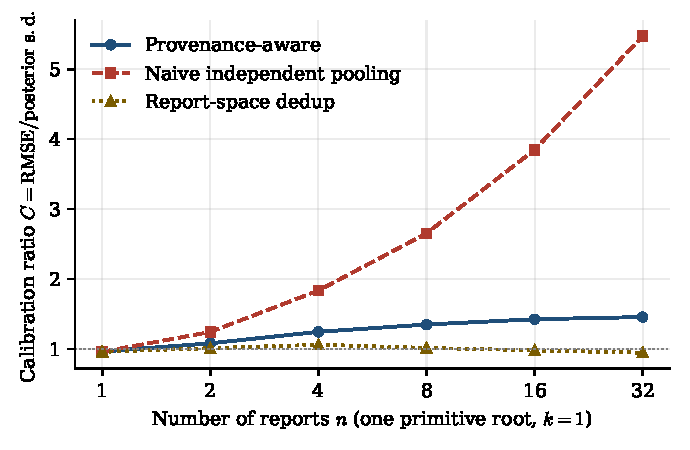
\includegraphics[width=.68\linewidth]{figures/fig5_calibration_empirical.pdf}
\caption{Empirical calibration ratio as report count increases with one
primitive evidence root ($k=1$), 300 evaluation worlds. The
provenance-aware posterior stays within a narrow band; the
independence-assuming posterior becomes progressively overconfident. The
report-space dedup baseline is shown for reference; see
Section~\ref{sec:emp-2x2} for its behavior under manipulated
representation.}
\label{fig:emp-calibration}
\end{figure}

\begin{figure}[t]
\centering
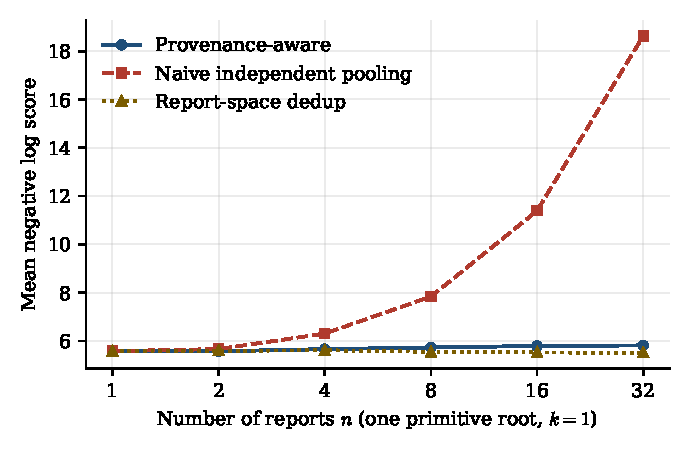
\includegraphics[width=.68\linewidth]{figures/fig6_logscore_empirical.pdf}
\caption{Mean negative log score against report count $n$, one primitive
evidence root, 300 evaluation worlds.}
\label{fig:emp-logscore-n}
\end{figure}

The residual drift in provenance-aware coverage away from the nominal 0.95
is not attributable to the shared-root correction itself;
Section~\ref{sec:emp-gamma} below identifies its source directly.

\subsection{Independent evidence roots restore information}
\label{sec:emp-roots}

The second question is the mirror image: when additional reports really
do carry new evidence, does the overconfidence disappear? Holding report
count fixed at $n=16$ and varying the number of independent
primitive roots $k\in\{1,2,4,8,16\}$ isolates report count from evidential
ancestry, the empirical analogue of Section~\ref{sec:sim-rootcount}'s
simulation; this root-multiplicity design is Grid~B, the second
confirmatory grid. At $k=1$ the two aggregators are far apart: naive coverage is
0.400 against provenance-aware's 0.860, and naive mean negative log score
is 11.39 against provenance-aware's 5.79. As $k$ rises toward $n$, this
gap closes monotonically, and at $k=16$, where every report has its own
root and the naive independence assumption is literally correct, the two
aggregators are statistically indistinguishable: coverage 0.927 against
0.927, mean negative log score 4.584 against 4.585, RMSE 23.49 against
23.49 with overlapping bootstrap intervals. The $k=1$ cell of this design
reproduces Grid~A's $n=16$ cell exactly, since it is the same underlying
data viewed from the other axis, which serves as an internal consistency
check on the analysis pipeline. Figure~\ref{fig:emp-logscore-k} shows mean
negative log score against $k$.

\begin{figure}[t]
\centering
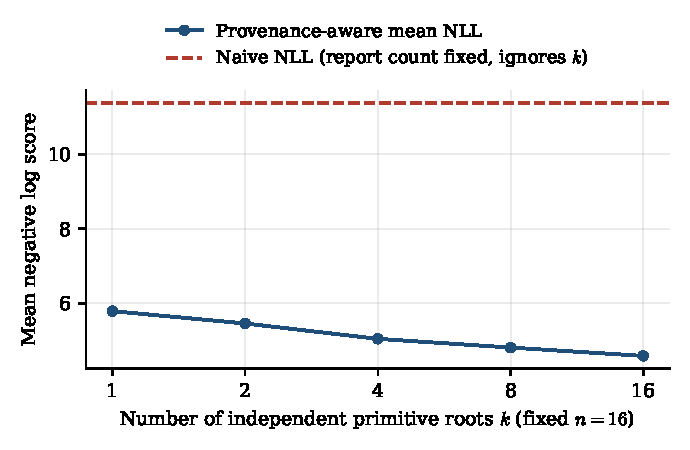
\includegraphics[width=.68\linewidth]{figures/fig7_roots_info_empirical.pdf}
\caption{Mean negative log score at fixed report count $n=16$ as the
number of independent primitive roots $k$ varies, 300 evaluation worlds.
Although the naive aggregator uses the same independence-based
uncertainty model for every $k$, its realized log score improves as
additional independent roots improve the accuracy of the pooled estimate;
what does not track $k$ is its assumed uncertainty, which is why its
calibration lags provenance-aware's until $k$ approaches $n$.}
\label{fig:emp-logscore-k}
\end{figure}

This result functions as a structural control on
Section~\ref{sec:emp-multiplicity}'s finding. The naive aggregator is not
simply penalized for having many reports; it is penalized specifically for
treating correlated reports as independent, and the penalty vanishes
exactly when that assumption becomes true. Report count alone does not
predict the naive-provenance gap; root count does.

\subsection{Correlated extraction errors and the information ceiling}
\label{sec:emp-gamma}

The third question concerns re-reading: how much can repeated extraction
from one fixed document actually add, and where does it stop? When
several agents independently extract information from a fixed noisy
source, additional agents can improve inference, but improvement should
exhibit diminishing returns toward a source-dependent ceiling; the
relevant empirical target is the existence and approximate level of that
ceiling. The independent-extraction specification underlying the
provenance-aware aggregator above assumes each report's extraction error
is drawn afresh. Grid~A's own data reject this assumption. The variance of the $m$-report
block mean, $\mathrm{Var}(\bar R_m-\Theta)$, computed across Grid~A's 300
worlds for $m\in\{1,2,4,8,16,32\}$, declines only slightly, from 9177 at
$m=1$ to 7510 at $m=32$, while the independent-extraction prediction
$\hat\sigma^2+\hat\nu^2/m$ falls from 7627 to 2678 over the same range and
lies outside the block mean's bootstrap confidence interval at every
$m\geq2$. Correlated replicate errors, the mechanism
Section~\ref{sec:correlated-extraction} anticipates for agents sharing a
base model, are the natural candidate: under that specification the
block-mean variance is
$\hat\sigma^2+\hat\gamma\hat\nu^2+(1-\hat\gamma)\hat\nu^2/m$ for a
correlation parameter $\hat\gamma$. This specification was already present
in the theoretical model; the decision to test it empirically was prompted
by the independent model's failure above, so the check that follows is
reported as an out-of-sample validation of an exploratory choice, not a
pre-registered confirmatory test.

Estimating $\hat\gamma$ exclusively on the 100 calibration worlds, from
the ratio of mean within-document report variance to $\hat\nu^2$, gives
$\hat\gamma_{\mathrm{cal}}=0.719$. The resulting prediction, with every
parameter estimated exclusively from the disjoint calibration split and
without fitting to Grid~A, falls inside Grid~A's bootstrap interval at all
six values of $m$, while the independent prediction remains outside for
$m\geq2$. An in-sample estimate of $\gamma$ from Grid~A's own
within-document variance gives 0.703, close to the calibration value and
consistent with a stable underlying parameter rather than an artifact of
either sample. Figure~\ref{fig:emp-precision} shows both predicted curves
against the empirical one.

\begin{figure}[t]
\centering
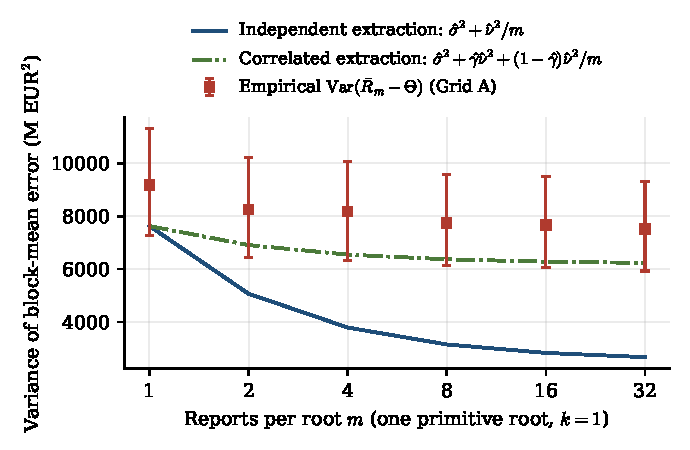
\includegraphics[width=.68\linewidth]{figures/fig8_precision_curve.pdf}
\caption{Empirical block-mean variance curve, 300 Grid~A evaluation
worlds, against the independent-extraction prediction
$\hat\sigma^2+\hat\nu^2/m$ and the correlated-extraction prediction using
$\hat\gamma_{\mathrm{cal}}=0.719$ estimated exclusively on the disjoint
calibration split. Both predictions use only calibration-fit parameters;
neither is tuned on the plotted data.}
\label{fig:emp-precision}
\end{figure}

An aggregator built on this specification, replacing
Proposition~\ref{prop:saturation}'s block precision with the
correlated-extraction form $J_m=m/\bigl(v+(m-1)c\bigr)$ for
$v=\hat\sigma^2+\hat\nu^2$ and $c=\hat\sigma^2+\hat\gamma_{\mathrm{cal}}\hat\nu^2$,
and using only calibration-fit parameters, restores coverage to between
0.940 and 0.953 across every value of $n$ in Grid~A, with calibration
ratio between 0.95 and 0.96 throughout, compared to the plain
provenance-aware aggregator's drift down to 0.850. This aggregator is
presented as an exploratory extension, not a confirmatory result, and is
kept visually separate from the confirmatory figures:
Figure~\ref{fig:emp-gamma-aggregator} shows naive, provenance-aware, and
provenance-with-correlated-extraction coverage and calibration ratio
together. A direct sensitivity check, subtracting the calibration-split
report bias of $-11.3$ from every report and re-running every aggregator,
changes no evaluation cell materially (the $k=16$ coverage in Grid~B moves
from 0.927 to 0.920), so the residual gap between provenance-aware
coverage and the nominal 0.95 is attributed to correlated extraction error
and heavy-tailed residuals rather than to bias. Extraction noise pooled
across Grid~A's root-0 reports departs visibly from normality in the
tails, with excess kurtosis 2.35 and 1.2\% of standardized residuals
beyond three standard deviations against 0.27\% expected under a normal
distribution (Figure~\ref{fig:emp-qq}), a further source of Gaussian
likelihood misspecification contributing to the remaining gap to nominal
coverage.

\begin{figure}[t]
\centering
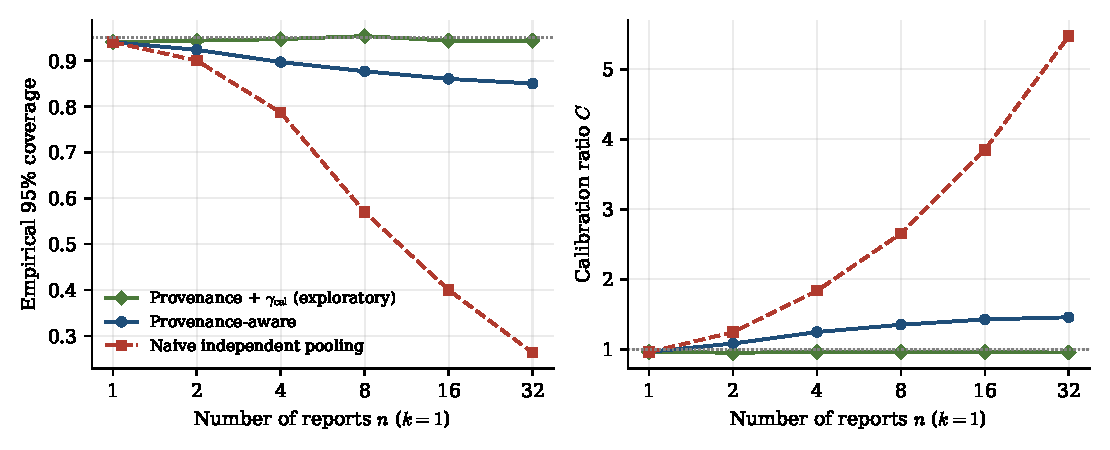
\includegraphics[width=\linewidth]{figures/fig10_gamma_exploratory.pdf}
\caption{Exploratory extension: naive, provenance-aware, and
provenance-aware with the correlated-extraction correction, coverage
(left) and calibration ratio (right) across Grid~A. Kept visually separate
from the confirmatory Figures~\ref{fig:emp-calibration} and~\ref{fig:emp-logscore-n}.}
\label{fig:emp-gamma-aggregator}
\end{figure}

\begin{figure}[t]
\centering
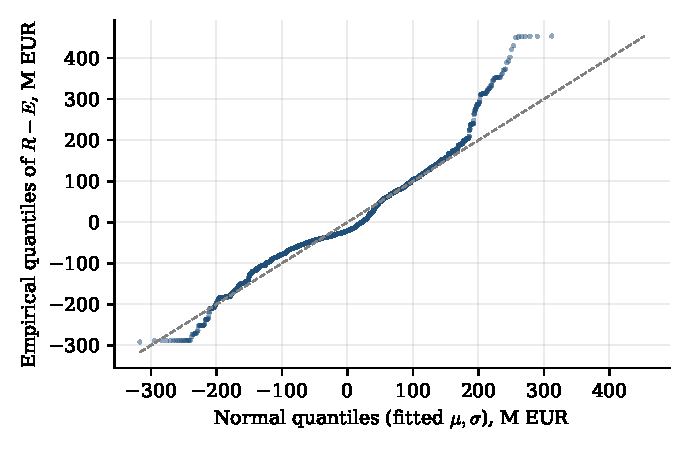
\includegraphics[width=.68\linewidth]{figures/fig9_extraction_noise_qq.pdf}
\caption{Quantile-quantile plot of extraction noise $R-E$ against a fitted
normal distribution, pooled over Grid~A's root-0 reports ($n=9600$).}
\label{fig:emp-qq}
\end{figure}

\subsection{Representation similarity does not identify evidential ancestry}
\label{sec:emp-2x2}

The final question is whether the reports themselves can reveal where
they came from: can a system tell, by inspecting report content, whether
the reports descend from one source or several? A report-space defense
should be misled if it identifies evidential
independence from semantic similarity rather than from ancestry itself,
the possibility Theorem~\ref{thm:non-identifiability} leaves open once
provenance is unavailable. A $2\times2$ design tests this directly. Every world generates
four independent evidence roots; ancestry is manipulated by which roots
feed a cell's four reports, shared for cells A and C, independent for
cells B and D. Representation is manipulated separately and only after
elicitation, through a controlled replacement of the textual rationale
channel that leaves the estimate and every evidential input unchanged: one
frozen prompt, identical across every cell, produces an estimate and a raw
rationale; a deterministic post-hoc renderer, which never reads the
report's estimate or raw rationale, then supplies the rationale text that
is actually embedded, drawn from one of two fixed template pools that
describe the task's common three-segment structure in different
vocabulary rather than paraphrasing any individual report's specific
content. Cells A and B receive one rendering style, C and D the other. An
earlier design that manipulated representation through the elicitation
prompt itself was found in a pilot to change extraction accuracy between
styles, confounding representation with extraction quality; the redesign
used here removes that confound by construction, since the estimate cannot
depend on a rendering step that never sees it (the earlier design and why
it was rejected are recorded in the supplementary experimental log).

Across 200 evaluation worlds, the effect of the representation
manipulation on the deduplication baseline's inferred cluster count is
$+1.425$ (paired bootstrap by world, 95\% CI $[1.363,1.485]$), computed as
the average cluster count in the two dissimilar-representation cells minus
the average in the two similar-representation cells. The effect of a
fourfold change in true root count is $+0.040$ (95\% CI
$[-0.045,0.120]$), computed the same way across the ancestry contrast. The
representation effect is large and precisely estimated, whereas the
ancestry effect is close to zero and statistically indistinguishable from
zero. A separate similarity check,
$\Delta_{BC}=\mathbb E[\cos(B)]-\mathbb E[\cos(C)]$, comparing
independent-root reports rendered alike against shared-root reports
rendered differently, gives $0.248$ (95\% CI $[0.236,0.259]$) on the
evaluation set, closely reproducing a pilot estimate of $0.242$
(95\% CI $[0.216,0.270]$) obtained on a disjoint set of 30 worlds before
the design was frozen.

\begin{figure}[t]
\centering
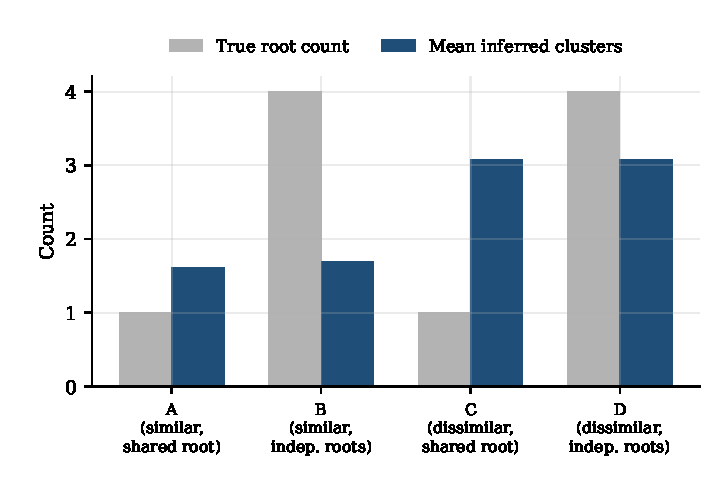
\includegraphics[width=.7\linewidth]{figures/fig12_cluster_counts.pdf}
\caption{True root count versus mean inferred cluster count for each of
the four design cells, 200 evaluation worlds. Cells sharing a
representation style (A, B) and cells sharing a dissimilar-representation
pairing (C, D) cluster together regardless of true ancestry.}
\label{fig:emp-clusters}
\end{figure}

Because cells A and C share identical evidence and identical estimates,
differing only in which representation was rendered downstream, the
contrast between them isolates representation's effect from every other
factor. Under the deduplication aggregator, this contrast moves every
downstream metric in the harmful direction with confidence intervals
excluding zero: coverage falls by $0.125$ ($[-0.175,-0.080]$), mean
negative log score rises by $0.223$ ($[0.099,0.373]$), and calibration
ratio rises by $0.416$ ($[0.333,0.513]$). The analogous contrast between
the independent-root cells, D minus B, shows no coverage or calibration
effect distinguishable from zero and a favorable shift in log score,
because for cell D the dissimilar rendering happens to coincide with the
cell's true independent structure rather than working against it. Naive
and provenance-aware aggregators are, as they should be, identical between
A and C and between B and D, since neither reads report content.

A threshold, chosen to balance mean log score equally across all four
cells on 60 calibration worlds disjoint from evaluation and frozen before
evaluation began, does not resolve the underlying conflict. The
false-merge rate is the fraction of different-root report pairs assigned
to the same cluster; the false-split rate is the fraction of same-root
report pairs assigned to different clusters. At this
threshold the false-merge rate in cell B is 0.622 and the false-split rate
in cell C is 0.846. Sweeping every cosine-similarity value that is
actually distinct in the evaluation data, so that every threshold capable
of producing a different clustering decision is covered exactly rather
than by a spaced grid, the minimum achievable value of the worse of the
two error rates is $\min_t\max\bigl(\mathrm{FMR}_B(t),\mathrm{FSR}_C(t)\bigr)=0.846$.
No threshold for this similarity-based clustering rule achieves low
false-merge and false-split error simultaneously on the observed
evaluation set. Figure~\ref{fig:emp-tradeoff} shows the false-merge and
false-split rates against each other across the swept range
(Figure~\ref{fig:emp-clusters}, above, shows mean inferred cluster count
against true root count), and Figure~\ref{fig:emp-coverage} shows coverage
by aggregator and cell.

\begin{figure}[t]
\centering
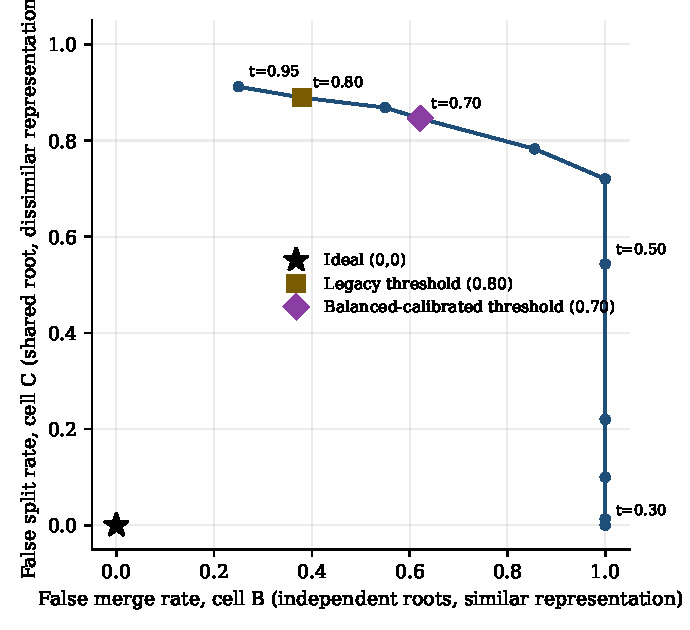
\includegraphics[width=.68\linewidth]{figures/fig11_tradeoff_curve.pdf}
\caption{False merge rate in cell B against false split rate in cell C
across the swept threshold range, 200 evaluation worlds. The legacy
threshold (0.80) and the balanced-calibrated threshold (0.70) are marked;
the ideal point (0,0) is far from the entire curve.}
\label{fig:emp-tradeoff}
\end{figure}

\begin{figure}[t]
\centering
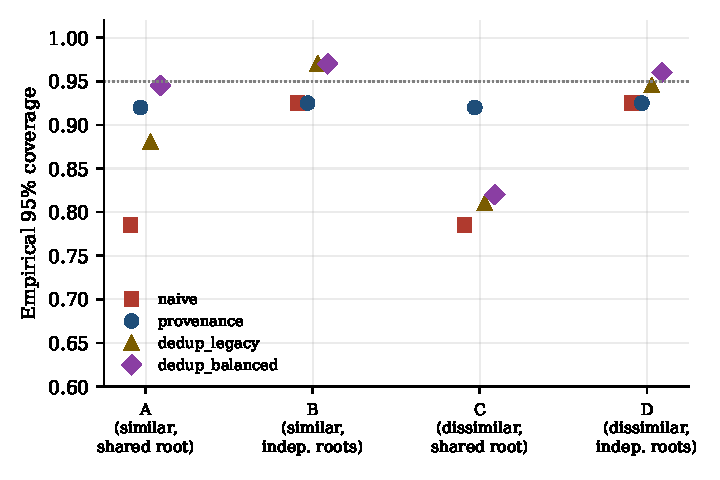
\includegraphics[width=.7\linewidth]{figures/fig13_coverage_by_cell.pdf}
\caption{Empirical 95\% coverage by aggregator and design cell, 200
evaluation worlds. Naive and provenance-aware are identical between cells
sharing true ancestry (A/C and B/D); the dedup aggregators are not.}
\label{fig:emp-coverage}
\end{figure}

This experiment is a controlled representation stress test: it establishes
that a controlled change to the textual rationale channel alone, holding
the latent state, the primitive evidence, the extraction process, and the
estimate fixed, can invert what report-only similarity implies about
evidential ancestry for one concrete mechanism (rationale embedding with
cosine-threshold clustering) on one task family. It illustrates the
report-only non-identifiability result of Theorem~\ref{thm:non-identifiability}
operationally; it does not establish that every report-space defense must
fail this way, nor does it characterize how often adversarial or
coincidental representation conflicts of this kind arise in deployed
systems.

\subsection{Summary of empirical findings}
\label{sec:emp-summary}

Three results, obtained from a single small language model reading
synthetic documents, are consistent with the paper's central claims.
Increasing report count at fixed evidential ancestry produces naive
overconfidence that grows with report count and is not accompanied by a
comparable accuracy gain, while a provenance-aware aggregator using the
same reports stays within a narrow calibration band; the naive-provenance
gap closes specifically as evidential ancestry, not report count, moves
toward independence. The same model's replicate extractions on a shared
document are more strongly correlated than an independent-extraction model
predicts, a pattern that a correlated-extraction refinement of the
shared-root model, evaluated out of sample, both explains and corrects. A
controlled design that manipulates representation similarity and
evidential ancestry independently shows that a concrete report-space
deduplication mechanism tracks the former far more strongly than the
latter, and that no similarity threshold resolves the resulting conflict
on the evaluation data.

These findings come with limitations that bound their scope. All data are
synthetic quarterly-revenue memos from one task family, generated to
control extraction difficulty precisely; no natural-language corpus or
real-world evidentiary claim is involved. A single main model was used
throughout, and no claim is made about how these effects scale across
model families; an alternative, larger model was evaluated and found
unsuitable for studying extraction noise at all, since it does not expose
an explicit sampling temperature and so cannot produce genuinely
independent replicate samples, a finding recorded with the full model
comparison in the supplementary experimental log rather than repeated
here. The $2\times2$ design's representation manipulation is a
deliberately artificial stress test and should not be read as a claim
about the rationale styles produced in ordinary use. The extraction-noise
distribution is heavy-tailed (excess kurtosis 2.35, with 1.2\% of
standardized residuals beyond three standard deviations against 0.27\%
under normality), so the Gaussian aggregators compared here are themselves
somewhat misspecified in the tails, a limitation that applies uniformly
across naive, provenance-aware, and correlated-extraction aggregators and
so does not favor any one of them. Finally, a pre-registered
informativeness gate from the pilot phase was not met on its literal
threshold; inspection traced the shortfall to genuine arithmetic
unreliability in the main model rather than to document ambiguity, and it
is retained here as a disclosed, uncorrected property of the studied
regime rather than treated as disqualifying, with the full gate protocol
and threshold recorded in the supplementary experimental log.

Code, the exact elicitation prompts, the frozen raw model outputs, the
calibration and evaluation world-id splits, and the analysis scripts
underlying every result in this section will be made publicly available.
The frozen Grid~A and Grid~B evaluation data are additionally packaged as
a standalone benchmark with a documented aggregator interface, a scoring
command, and reference baseline adapters, so that other dependence-aware
aggregation methods can be evaluated on the same report-multiplicity and
root-multiplicity axes without rerunning any model calls.
Every reported table and figure in this section can be reproduced from
the archived, frozen model outputs without access to the Anthropic API or
any other hosted model provider. (The synthetic-model validation of
Section~\ref{sec:simulation} involves no model calls at all and is
separately reproducible from its fixed simulation seed.) Rerunning the live elicitation calls that generated those
outputs is possible for a reader with valid API credentials but
constitutes a replication of the experiment rather than a guaranteed exact
computational reproduction, since hosted model providers can update model
weights or serving behavior behind a fixed model identifier without
notice.
